\documentclass[../thesis.tex]{subfiles}

\begin{document}


% \section{Traditional Motion Planning (not sure)}


%% Meta controller in DRL, H-DRL

\section{Deep Reinforcement Learning (DRL)} 
% \label{sec:mdrl-background}
% \subsection{}

%% general introduction of RL notation and several useful function (Q, V, A, mu, ...) %%%

We consider a standard Reinforcement Learning (RL) setup, where an agent operates in an environment ${E}$. At each discrete time step $t$, the agent observes a state $s_t \in \mathcal{S}$, picks an action $a_t \in \mathcal{A}$, and receives a scalar reward $r(s_t, a_t) \in \mathbb{R}$ from the environment. The return $R_t = \sum^T_{i=t} \gamma^{(i-t)}r(s_i,a_i)$ is defined as total discounted future reward at time step $t$, with $\gamma$ being a discount factor $\in [0,1]$. The objective of the agent is to learn a policy that eventually maximizes the expected return, as shown below:

\begin{align}
\centering
J = \mathbb{E}_{s_i, r_i \sim E~, a_i \sim \pi}[R_1] \label{equ:obj-func} 
\end{align}

The learned policy, $\pi$, can be formulated as either stochastic $\pi(a|s) = \mathbb{P}(a|s)$, or deterministic $a = \mu(s)$. The value function $V^{\pi}$ and action-value function $Q^{\pi}$ describe the expected return for each state and state-action pair upon following a policy $\pi$. 

\begin{align}
V^\pi(s_t) &= \mathbb{E}_{r_{i \geq t}, s_{i > t} \sim E, a_{i \geq t} \sim \pi} [R_t | a_t, s_t] \\
Q^\pi(s_t, a_t) &= \mathbb{E}_{r_{i \geq t}, s_{i > t} \sim E} [r(s_t, a_t) \nonumber \\
&\qquad + \gamma \mathbb{E}_{a_{i > t} \sim \pi} [Q^\pi(s_{t+1}, a_{t+1})]]
\end{align}

Finally, an advantage function $A^{\pi}(s_t,a_t)$ is defined as the additional reward or advantage that the agent will have for executing some action $a_t$ at state $s_t$ and its is given by $A^{\pi}(s_t,a_t) = Q^\pi(s_t, a_t) - V^\pi(s_t)$. 

%% Deep architecture on RL -> DRL! %%%

In high dimensional state/action space, these functions are usually approximated by a suitable parametrization. Accordingly, we define $\theta^Q$, $\theta^V$, $\theta^A$, $\theta^\pi$, and $\theta^\mu$ as the parameters for approximating $Q$, $V$, $A$, $\pi$, and $\mu$ functions, respectively. It was generally believed that using non-linear function approximators for both $Q$ and $V$ functions would lead to unstable learning in practice. Recently, \citet{mnih2013playing} applied two novel modifications, namely \textit{replay buffer} and \textit{target network}, to stabilize the learning with deep nets. Later, several variants were introduced that exploited deep architectures and extended to learning tasks with continuous actions \cite{DBLP:journals/corr/LillicrapHPHETS15,A3C,CDQN,TRPO}. 

To exhaustively analyze the effect of multi-sensor input and the new stochastic regularization technique, we picked two algorithms, namely DDPG and NAF. It is worth noting that the two algorithms are very different, with DDPG being an off-policy actor-critic method and NAF an off-policy value-based one. By augmenting these two algorithms, we highlight that any DRL algorithm, modified appropriately, can benefit from using multiple inputs. Before introducing the multi-modal architecture, we briefly summarize the two algorithms below.


\subsection{Normalized Advantage Function (NAF)} 
\label{sec:CDQN}

%%% Q-learning %%%
Q-learning \cite{sutton1999policy} is an off-policy model-free algorithm, where agent learns an approximated $Q$ function, and follows a greedy policy $\mu(s)=\arg\max_aQ(s,a)$ at each step. The objective function (\ref{equ:obj-func}) can be reached by minimizing the square loss Bellman error

\begin{align}
\centering
L = \frac{1}{N} \sum_i^N (y_i-Q(s_i,a_i|\theta^Q))^2
\end{align}

where target $y_i$ is defined as $r(s_i,a_i) + \gamma Q(s_{i+1},\mu(s_{i+1}))$.

%%% DQN and C-DQN %%%

Deep Q-Network(DQN) parametrized $Q$ function with deep architecture\cite{mnih2013playing}, and has been shown to emulate human performance \cite{mnih2015human} in many Atari games using just image pixels as input. However, in all of these games, action choices are limited and discrete. Recently, \citet{CDQN} proposed a continuous variant of Deep Q-Learning by a clever network construction. The $Q$ network, which they called Normalized Advantage Function (NAF), parameterized the advantage function quadratically over the action space, and is weighted by non-linear feature of states. 
\begin{align}
\centering
Q(s,a|\theta^Q) &= A(s,a | \theta^\mu, \theta^L) + V(s|\theta^V) \\
A(s,a | \theta^\mu, \theta^L) &= -\frac{1}{2}(a-\mu(s|\theta^\mu))^T P(s|\theta^L)\nonumber \\
&\qquad \qquad \qquad(a-\mu(s|\theta^\mu)) \label{equ:NAF} \\
P(s|\theta^L) &= L(s|\theta^L)^TL(s|\theta^L) \label{equ:P}
\end{align}
During run-time, the greedy policy can be performed by simply taking the output of sub-network $a = \mu(s|\theta^\mu)$. The data flow at forward prediction and back-propagation steps are shown in Fig. \ref{fig:CDQN-DDPG} (a) and (b), respectively.

\begin{figure}[t]
	\begin{center}
	\centerline{
\includegraphics[width=0.8\columnwidth,trim= 80 900 110 70, clip=true]{./MultimodalDRL/fig/naf_ddpg}}
	\caption{Schematic illustration of (a) forward and (b) back-propagation for NAF, and (c) forward and (d) back-propagation for DDPG. Green modules are functions approximated with Deep Nets.}
	\label{fig:CDQN-DDPG}
	\end{center}
\end{figure} 

\subsection{Deep Deterministic Policy Gradient (DDPG)}
%%% Actor-Critic and DPG %%%
An alternative approach to continuous RL tasks was the use of an actor-critic framework, which maintains an explicit policy function, called \textit{actor}, and an action-value function called as \textit{critic}. In \citet{dpg}, a novel \emph{deterministic} policy gradient (DPG) approach was proposed and it was shown that deterministic policy gradients have a model-free form and follow the gradient of the action-value function. 

\begin{equation}
\nabla_{\theta^\mu} J = \mathbb{E}[\nabla_a Q(s,a|\theta^Q) \nabla_a \mu(s)]
\label{dpg}
\end{equation}
\citet{dpg} proved that using the policy gradient calculated in (\ref{dpg}) to update model parameters leads to the maximum expected reward.

%%% DDPG %%%
Building on this result, \citet{DBLP:journals/corr/LillicrapHPHETS15} proposed an extension of DPG with deep architecture to generalize their prior success with discrete action spaces \cite{mnih2015human} onto continuous spaces. Using the DPG, an off-policy algorithm was developed to estimate the $Q$ function using a differentiable function approximator. Similar techniques as in \cite{mnih2015human} were utilized for stable learning. In order to explore the full state and action space, an exploration policy was constructed by adding Ornstein-Uhlenbeck noise process \cite{uhlenbeck1930theory}. In short, actions are chosen stochastically but a deterministic policy gradient is learned. The data flow for prediction and back-propagation steps are shown in Fig. \ref{fig:CDQN-DDPG} (c) and (d), respectively.


%%%%%%%%%%%%%%%%%%%%%%%%%%%%%%%%%%%%%%%%%%%%%%%%%%%%%%%%%%%%%%%%%%%%%%%%%%%%%%%%%%%%%%%%%%%%%%%%%%%%%%%%%%%%%%%%%%%%%%

\section{Deep Inverse Reinforcement Learning (DIRL)} 
\label{sec:dirl}

%%% Formulation of IRL %%%

\begin{figure}[t]
	\begin{center}
		\centerline{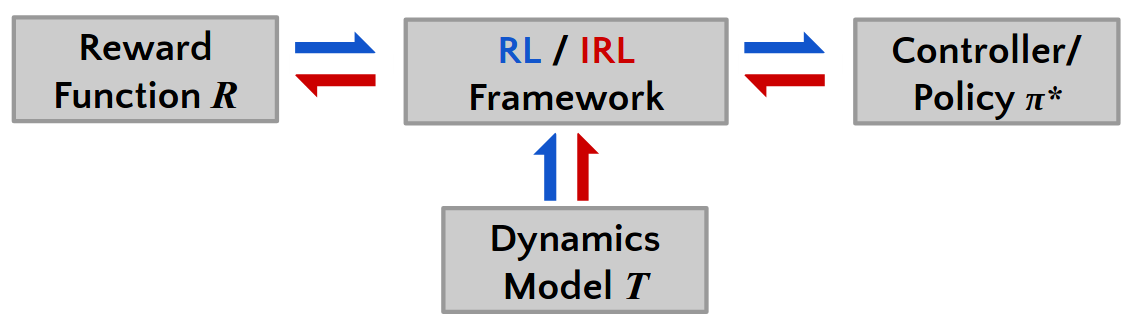
\includegraphics[width=0.5\columnwidth]{./DIRL/fig/irl_rl_pipeline.png}}
		\caption{The block diagram of reinforcement learning and inverse reinforcement learning.}
		\label{fig:irl_rl}
	\end{center}
\end{figure} 

As shown in Fig. \ref{fig:irl_rl},
in the standard reinforcement learning, we are interested in learning the optimal policy that maximizes the total expected reward collected from the environment. However, for the situation where the consequence of the policy is relatively easy to observe, yet designing a cost function can be nontrivial and often requires lots of handy tuning, we can formulate the problem by solving the standard reinforcement learning \textit{inversely}. (See Fig. X) The problem is thereby called \textit{inverse} reinforcement learning (IRL) or Learning from demonstration (LfD) \todo{check this}. Given a set of expert demonstration $D=\left\{ \xi_i \right\}_{i=1}^{N}$, where each trajectory $\xi_i$ consists of a sequence of state-action pair $\xi_i = \left\{ (s_j, a_j) \right\}_{j=1}^{K}$, the goal is to infer the underlying reward function that lead to the optimal policy $\pi$. The reward function $r$ is parametrized by $\theta$.

%%% IRL as a MAP Formulation %%%
% Under the standard definition of Markov Decision Process (MDP). 
Modeling the behavior of the export naturally lead to different formulation of the objective function. If the problem is cast as a maximum margin structured prediction framework \cite{ratliff2006maximum}, the resulting objective function leads to the form of

\begin{align}
L(\theta) = \frac{1}{N} \sum^{N}_{i=1} \beta_i ( \max_{\mu \in \mathbb{G}_i}(\theta^T F_i + l_i^T)\mu - \theta^TF_i\mu_i )^q +  \frac{\lambda}{2} \| \theta \|^2
\end{align}

where $\mu_i$, $F_i$, and $l_i$ represent the state visited frequencies (SVF), feature matrix, and margin loss vector of the $i^{th}$ trajectory, respectively.

%%% ME-IRL %%%

An alternative approach is to explicitly loosen the optimality assumption of expert behavior by modeling the demonstration with a stochastic policy. \citet{ziebart2008maximum} reformulates the problem under the principle of maximum entropy. The resulting algorithm, known as maximum entropy IRL (ME-IRL), assumes the preference of each trajectory is exponentially proportional to its total accumulated rewards. The gradient of the objective function under linear reward function is simply the difference between the expected empirical feature counts and the learner's expected feature counts. 

%%% ME-DIRL %%%

\begin{figure}[t]
	\begin{center}
		\centerline{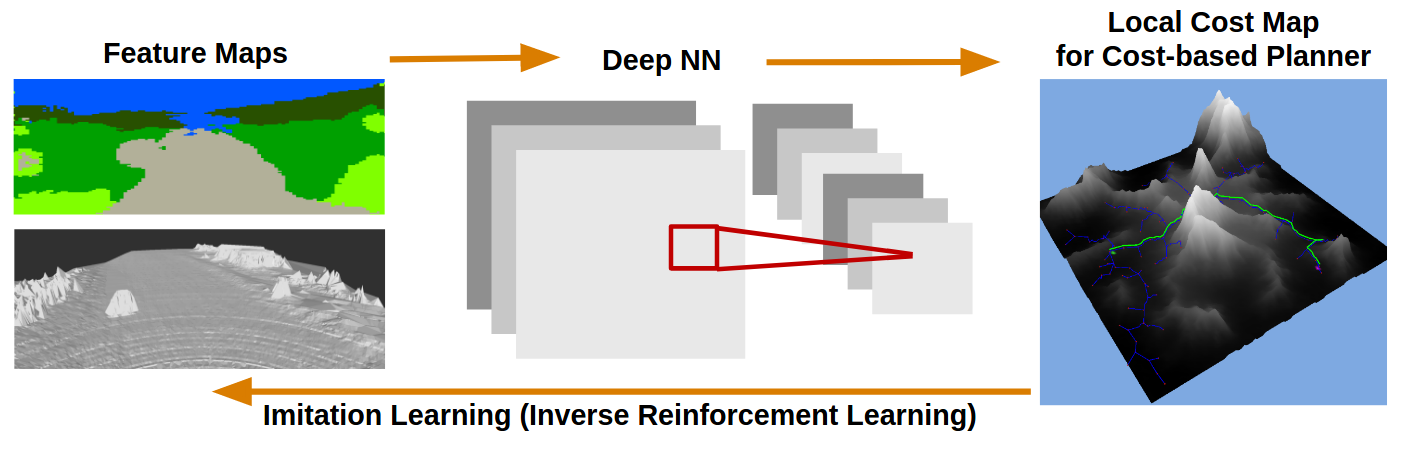
\includegraphics[width=0.9\columnwidth]{./DIRL/fig/dirl_pipeline.png}}
		\caption{Schematic illustration of deep inverse reinforcement learning.}
		\label{fig:dirl_diagram}
	\end{center}
\end{figure} 

Recently, \citet{wulfmeier2015maximum} shows that the gradient calculation in ME-IRL can be naturally extended to the back-propagation in the standard deep supervised learning. By framing the problem within the standard Bayesian inference as MAP estimation. The objective function can now be defined as the negative log-likelihood of the observed demonstrations. 

\begin{align}
L(\theta) = \log P(D,\theta|r) = \log P(D|r) + \log P(\theta) \label{equ:irl_obj}
\end{align}

The objective function can be interpreted as the data term $L_{D}$ and a standard weight decay term $L_{\theta}$ as model regularization. The gradient of the former term is simply:

\begin{align}
\frac{\partial L_D}{\partial \theta} &= \frac{\partial L_D}{\partial r} \frac{\partial r}{\partial \theta} \\
&= (\mu_D - \mathbb{E}[\mu]) \cdot \frac{\partial r}{\partial \theta}
\end{align}

Since the reward function is approximated by a deep network, the latter term $\partial r / \partial \theta$ fits with the the back-propagation, and the objective function can be optimized using gradient-based approach. This framework, called deep maximum entropy deep inverse reinforcement learning (ME-DIRL or simply DIRL) has shown to successfully apply in urban autonomous navigation \cite{wulfmeier2016watch}. The use of deep neural net provides a more powerful non-linear reward function approximator. The schematic illustration of the DIRL is summarized in Fig. \ref{fig:dirl_diagram}.

%%% Other Non linear IRL %%%
% An alternative choice for non-linear IRL is to use Grassian process \cite{levine2011nonlinear}. 

%%% Connections to MMP and MEIRL %%%
% However, the two formulation can be generalized in a unification. 


\end{document}
